%%%%%%%%%%%%%%%%%%%%%%%%%%%%%%%%%%%%%%%%%
% fphw Assignment
% LaTeX Template
% Version 1.0 (27/04/2019)
%
% This template originates from:
% https://www.LaTeXTemplates.com
%
% Authors:
% Class by Felipe Portales-Oliva (f.portales.oliva@gmail.com) with template 
% content and modifications by Vel (vel@LaTeXTemplates.com)
%
% Template (this file) License:
% CC BY-NC-SA 3.0 (http://creativecommons.org/licenses/by-nc-sa/3.0/)
%
%%%%%%%%%%%%%%%%%%%%%%%%%%%%%%%%%%%%%%%%%

%----------------------------------------------------------------------------------------
%	PACKAGES AND OTHER DOCUMENT CONFIGURATIONS
%----------------------------------------------------------------------------------------

\documentclass[
  12pt,
  %fleqn, % Default font size, values between 10pt-12pt are allowed
  %letterpaper, % Uncomment for US letter paper size
  %spanish, % Uncomment for Spanish
]{fphw}

% Template-specific packages
\usepackage[utf8]{inputenc} % Required for inputting international characters
\usepackage[T1]{fontenc} % Output font encoding for international characters
\usepackage{mathpazo} % Use the Palatino font

\usepackage{graphicx} % Required for including images

\usepackage{booktabs} % Required for better horizontal rules in tables

\usepackage{listings} % Required for insertion of code

\usepackage{enumerate} % To modify the enumerate environment

\usepackage{enumitem}

\usepackage{amsmath}

\usepackage{mathtools,amsthm}

\usepackage{float}

\usepackage{listings}

\usepackage{hyperref}

\usepackage{tikz}
\usetikzlibrary{patterns}

\lstdefinelanguage{R}{
  keywords={if, else, repeat, while, function, for, in, next, break},
  otherkeywords={TRUE, FALSE, NULL, NA, Inf, NaN},
  sensitive=true,
  morecomment=[l]\#,
  morestring=[b]",
}

\newcommand{\E}{\mathbb{E}}
\newcommand{\Var}{\operatorname{Var}}
\newcommand{\R}{\mathbb{R}}
\newcommand{\norm}[1]{\left\lVert #1 \right\rVert}


%----------------------------------------------------------------------------------------
%	ASSIGNMENT INFORMATION
%----------------------------------------------------------------------------------------

\title{Homework \#7} % Assignment title

\author{Shizhe Zhang} % Student name

\date{\today} % Due date

\institute{University of California, Berkeley \\ Department of Statistics} % Institute or school name

\class{EECS 227AT} % Course or class name

\professor{Gireeja Ranade} % Professor or teacher in charge of the assignment

%----------------------------------------------------------------------------------------

\begin{document}

\maketitle % Output the assignment title, created automatically using the information in the custom commands above

%----------------------------------------------------------------------------------------
%	ASSIGNMENT CONTENT
%----------------------------------------------------------------------------------------
\section*{Problem 1. Convex or Concave}

Determine whether the following functions are convex, strictly convex, concave, strictly concave, both or neither.

\begin{enumerate}
\item[(a)] $f(x) = e^x - 1$ on $\mathbb{R}$.

\item[(b)] $f(x_1, x_2) = x_1 x_2$ on $\mathbb{R}_{++}^2$, i.e., when $x_1 > 0$ and $x_2 > 0$.

\item[(c)] The log-likelihood of a set of points $\{x_1, . . . , x_n\}$ that are normally distributed with mean $\mu$ and finite variance $\sigma > 0$ is given by:

\[
f(\mu, \sigma) =
n \log \left(
\frac{1}{\sqrt{2\pi\sigma}}
\right)
-
\frac{1}{2\sigma^2}
\sum_{i=1}^{n} (x_i - \mu)^2
\]

\begin{enumerate}

\item[(i)] Show that if we view the log likelihood for fixed $\sigma$ as a function of the mean, i.e.

\[
g(\mu) =
n \log
\left(
\frac{1}{\sqrt{2\pi\sigma}}
\right)
-
\frac{1}{2\sigma^2}
\sum_{i=1}^{n} (x_i - \mu)^2
\]

then $g$ is strictly concave (equivalently, we say $f$ is strictly concave in $\mu$).

\item[(ii)] Show that if we view the log likelihood for fixed $\mu$ as a function of the inverse of the variance, i.e.

\[
h(z) =
n \log
\left(
\frac{\sqrt{z}}{\sqrt{2\pi}}
\right)
-
\frac{z}{2}
\sum_{i=1}^{n} (x_i - \mu)^2
\]

then $h$ is strictly concave (equivalently, we say $f$ is strictly concave in $z = \frac{1}{\sigma^2}$). Note that we have used the dummy variable $z$ to denote $\frac{1}{\sigma^2}$.

\item[(iii)] Show that $f$ is not jointly concave in $\mu$, $\frac{1}{\sigma^2}$. HINT: We say a function $w(\vec{x}, \vec{y})$ with $\vec{x} \in \mathbb{R}^m$ and $\vec{y} \in \mathbb{R}^n$ is jointly convex if

\[
w(\lambda(\vec{x}_1, \vec{y}_1) + (1-\lambda)(\vec{x}_2, \vec{y}_2))
\le
\lambda w((\vec{x}_1, \vec{y}_1)) + (1-\lambda) w((\vec{x}_2, \vec{y}_2)).
\]

This is the same as letting $\vec{z} = (\vec{x}, \vec{y})$ and saying $f$ is convex in $\vec{z}$. We can define joint concavity in a similar fashion by reversing the inequalities.

\end{enumerate}

\item[(d)] $f(x) = \log(1 + e^x)$. Note that this implies that $g(x) = -f(x) = \log\left(\frac{1}{1+e^x}\right)$ is concave. Compare this to $h(x) = \frac{1}{1+e^x}$, is $h(x)$ convex or concave?

\end{enumerate}

\subsection*{Answer}

\begin{enumerate}

\item[(a)] 
$f(x) = e^x - 1$.

We compute derivatives:
\[
f'(x) = e^x, \qquad f''(x) = e^x.
\]

Since $e^x > 0$ for all $x \in \mathbb{R}$, we have
\[
f''(x) > 0 \quad \forall x.
\]

Therefore $f$ is strictly convex on $\mathbb{R}$.

\item[(b)] 
$f(x_1,x_2)=x_1x_2$ on $\mathbb{R}_{++}^2$.

Compute the Hessian:
\[
\nabla^2 f(x) =
\begin{bmatrix}
0 & 1 \\
1 & 0
\end{bmatrix}.
\]

The eigenvalues of this matrix satisfy
\[
\det
\begin{bmatrix}
-\lambda & 1 \\
1 & -\lambda
\end{bmatrix}
= \lambda^2 -1 =0
\]

so
\[
\lambda = \pm 1.
\]

Thus the Hessian has both positive and negative eigenvalues, meaning it is indefinite. Therefore the function is neither convex nor concave on $\mathbb{R}_{++}^2$.

\item[(c)]

\begin{enumerate}

\item[(i)]
For fixed $\sigma$, the log-likelihood as a function of $\mu$ is

\[
g(\mu)=
n\log\left(\frac{1}{\sqrt{2\pi\sigma}}\right)
-
\frac{1}{2\sigma^2}\sum_{i=1}^n (x_i-\mu)^2.
\]

The first term is constant in $\mu$. Let

\[
S(\mu)=\sum_{i=1}^n (x_i-\mu)^2.
\]

Expand:

\[
S(\mu)=\sum_{i=1}^n(x_i^2-2x_i\mu+\mu^2)
= C -2\mu\sum_{i=1}^n x_i + n\mu^2
\]

where $C$ is constant.

Thus

\[
g(\mu)=\text{const} - \frac{1}{2\sigma^2}(n\mu^2 -2\mu\sum x_i + C).
\]

Compute derivatives:

\[
g'(\mu)=\frac{1}{\sigma^2}\sum_{i=1}^n (x_i-\mu),
\]

\[
g''(\mu)= -\frac{n}{\sigma^2}.
\]

Since $\sigma>0$,

\[
g''(\mu)<0.
\]

Therefore $g$ is strictly concave in $\mu$.

\item[(ii)]

\[
h(z)=
\frac{n}{2}\log z - \frac{n}{2}\log(2\pi)
-
\frac{z}{2}\sum_{i=1}^n (x_i-\mu)^2.
\]

Compute derivatives.

First derivative:

\[
h'(z)=\frac{n}{2z}-\frac{1}{2}\sum_{i=1}^n (x_i-\mu)^2.
\]

Second derivative:

\[
h''(z)= -\frac{n}{2z^2}.
\]

For $z>0$,

\[
h''(z)<0.
\]

Thus $h$ is strictly concave.


\item[(iii)]

Rewrite the function using $z=\frac{1}{\sigma^2}$:

\[
f(\mu,z)=
\frac{n}{2}\log z
-
\frac{z}{2}\sum_{i=1}^n (x_i-\mu)^2
+ \text{constant}.
\]

Expand the quadratic term:

\[
\sum_{i=1}^n (x_i-\mu)^2
=
\sum x_i^2 -2\mu\sum x_i + n\mu^2.
\]

Thus

\[
f(\mu,z)=
\frac{n}{2}\log z
-
\frac{z}{2}
(\sum x_i^2 -2\mu\sum x_i + n\mu^2)
+ \text{constant}.
\]

The term $zn\mu^2$ creates interaction between $\mu$ and $z$.

Compute the mixed second derivative:

\[
\frac{\partial^2 f}{\partial \mu \partial z}
=
\sum_{i=1}^n (x_i-\mu).
\]

Because the Hessian matrix contains mixed terms and is not negative semidefinite for all $(\mu,z)$, the function is not jointly concave.

\end{enumerate}

\bigskip

\item[(d)]

\[
f(x)=\log(1+e^x)
\]

Compute derivatives.

First derivative:

\[
f'(x)=\frac{e^x}{1+e^x}.
\]

Second derivative:

\[
f''(x)=\frac{e^x}{(1+e^x)^2}.
\]

Since $e^x>0$,

\[
f''(x)>0.
\]

Thus $f$ is convex.

Now consider

\[
h(x)=\frac{1}{1+e^x}.
\]

First derivative:

\[
h'(x)= -\frac{e^x}{(1+e^x)^2}.
\]

Second derivative:

\[
h''(x)=
\frac{e^x(e^x-1)}{(1+e^x)^3}.
\]


\[
h''(x)
\begin{cases}
<0 & x<0 \\
=0 & x=0 \\
>0 & x>0
\end{cases}
\]

Thus the curvature changes sign.
\end{enumerate}

%----------------------------------------------------------------------------------------
\section*{Problem 2. Convex and strictly convex functions}

\begin{enumerate}

\item[(a)] Recall that a function $f : \mathbb{R}^n \rightarrow \mathbb{R}$ is said to be strictly convex if it satisfies Jensen’s inequality with strict inequality, i.e., $\forall \vec{x} \ne \vec{y} \in \mathbb{R}^n$ and $\forall t \in (0,1)$, we have

\[
f(t\vec{x} + (1-t)\vec{y}) < t f(\vec{x}) + (1-t) f(\vec{y})
\]

Show that for a strictly convex function $f : \mathbb{R}^n \rightarrow \mathbb{R}$, the problem

\[
\min_{\vec{x} \in \mathbb{R}^n} f(\vec{x})
\]

has at most one solution.

HINT: Try to argue by contradiction assuming that there are two solutions $\vec{x}_1$, $\vec{x}_2$ which achieve the minimum value. Argue that using these two points you can find another point in $\mathbb{R}^n$ with strictly smaller function value.

\item[(b)] Prove that for all convex optimization problems $\min_{\vec{x} \in X} f(\vec{x})$, where $f$ is a convex function and $X$ is a convex set, all local minima are global minima. You may not assume that $f$ is differentiable.

HINT: Start with assuming $\vec{x}^\star$ is a local minimum that is not global, and $\tilde{x}$ is a global minimum. Use the definition of the convexity of a function to prove by contradiction.

\end{enumerate}

\subsection*{Answer}
\begin{enumerate}

\item[(a)]

Assume for contradiction that the problem
\[
\min_{\vec{x} \in \mathbb{R}^n} f(\vec{x})
\]
has two distinct minimizers $\vec{x}_1 \neq \vec{x}_2$.

Since both achieve the minimum value,
\[
f(\vec{x}_1) = f(\vec{x}_2) = f^\star.
\]

Because $f$ is strictly convex, for any $t \in (0,1)$ we have
\[
f(t\vec{x}_1 + (1-t)\vec{x}_2)
<
t f(\vec{x}_1) + (1-t) f(\vec{x}_2).
\]

Substituting $f(\vec{x}_1) = f(\vec{x}_2) = f^\star$ gives
\[
f(t\vec{x}_1 + (1-t)\vec{x}_2)
<
t f^\star + (1-t) f^\star
=
f^\star.
\]

Thus
\[
f(t\vec{x}_1 + (1-t)\vec{x}_2) < f^\star,
\]
which contradicts the fact that $f^\star$ is the minimum value.


\item[(b)]

Consider the convex optimization problem
\[
\min_{\vec{x} \in X} f(\vec{x}),
\]
where $f$ is convex and $X$ is a convex set.

Assume $\vec{x}^\star$ is a local minimum but not a global minimum. Then there exists some $\tilde{x} \in X$ such that
\[
f(\tilde{x}) < f(\vec{x}^\star).
\]

Since $X$ is convex, for any $t \in (0,1)$ the point
\[
\vec{x}_t = (1-t)\vec{x}^\star + t\tilde{x}
\]
also lies in $X$.

Using convexity of $f$,
\[
f(\vec{x}_t)
\le
(1-t)f(\vec{x}^\star) + t f(\tilde{x}).
\]

Since $f(\tilde{x}) < f(\vec{x}^\star)$, we obtain
\[
(1-t)f(\vec{x}^\star) + t f(\tilde{x})
<
(1-t)f(\vec{x}^\star) + t f(\vec{x}^\star)
=
f(\vec{x}^\star).
\]

Thus
\[
f(\vec{x}_t) < f(\vec{x}^\star).
\]

For sufficiently small $t$, the point $\vec{x}_t$ can be made arbitrarily close to $\vec{x}^\star$. This contradicts the assumption that $\vec{x}^\star$ is a local minimum.

Therefore our assumption is false, and every local minimum must be a global minimum.

\end{enumerate}
%----------------------------------------------------------------------------------------

\newpage
\section*{Problem 3. Quadratic inequalities.}

Consider the set $S$ defined by the following inequalities:

\[
(x_1 \ge -x_2 + 1 \ \text{and} \ x_1 \le 0)
\ \text{or} \
(x_1 \le -x_2 + 1 \ \text{and} \ x_1 \ge 0).
\]

To be more precise,

\[
S_1 = \{ \vec{x} \in \mathbb{R}^2 \mid x_1 \ge -x_2 + 1, \ x_1 \le 0 \}
\]

\[
S_2 = \{ \vec{x} \in \mathbb{R}^2 \mid x_1 \le -x_2 + 1, \ x_1 \ge 0 \}
\]

\[
S = S_1 \cup S_2.
\]

\begin{enumerate}

\item[(a)] Draw the set $S$. Is it convex?

\item[(b)] Show that the set $S$ can be described as a single quadratic inequality of the form

\[
q(\vec{x}) = \vec{x}^T A \vec{x} + 2\vec{b}^T \vec{x} + c \le 0
\]

for matrix $A = A^T \in \mathbb{R}^{2\times2}$, $\vec{b} \in \mathbb{R}^2$ and $c \in \mathbb{R}$ i.e $S$ can be written as

\[
S = \{ \vec{x} \in \mathbb{R}^2 \mid q(\vec{x}) \le 0 \}.
\]

Find $A$, $\vec{b}$, $c$.

Hint: Can you combine the constraints to make one quadratic constraint?

\item[(c)] The convex hull of a set $A \subseteq \mathbb{R}^n$ is the set of all convex combinations of points in $A$, i.e.,

\[
\text{conv}(A) =
\left\{
\sum_{i=1}^{k} \theta_i \vec{x}_i
\mid
k \in \mathbb{N}, \theta_1,...,\theta_k \ge 0,
\sum_{i=1}^{k}\theta_i = 1,
\vec{x}_1,...,\vec{x}_k \in A
\right\}.
\]

What is the convex hull of $S$?

\item[(d)] We will now consider some convex optimization problems over $S_1$ that illustrate the role of the constraints in the optimization problem. For each of the following optimization problems find the optimal point, $\vec{x}^\ast$. Describe the constraints that are active in attaining the optimal value.

\begin{enumerate}

\item[(i)] Minimize $f(\vec{x}) = (x_1 + 1)^2 + (x_2 - 3)^2$ subject to $\vec{x} \in S_1$.

\item[(ii)] Minimize $f(\vec{x}) = (x_1 + 2)^2 + (x_2 - 2)^2$ subject to $\vec{x} \in S_1$.

\item[(iii)] Minimize $f(\vec{x}) = x_1^2 + x_2^2$ subject to $\vec{x} \in S_1$.

\end{enumerate}
\end{enumerate}

\subsection*{Answer}
\begin{enumerate}

\item[(a)]


Consider
\[
(-1,2)\in S_1, \qquad (1,0)\in S_2
\]
belong to $S$, but their midpoint
\[
(0,1)
\]
does not satisfy either set of inequalities strictly defining the regions in the union.
    
\begin{center}
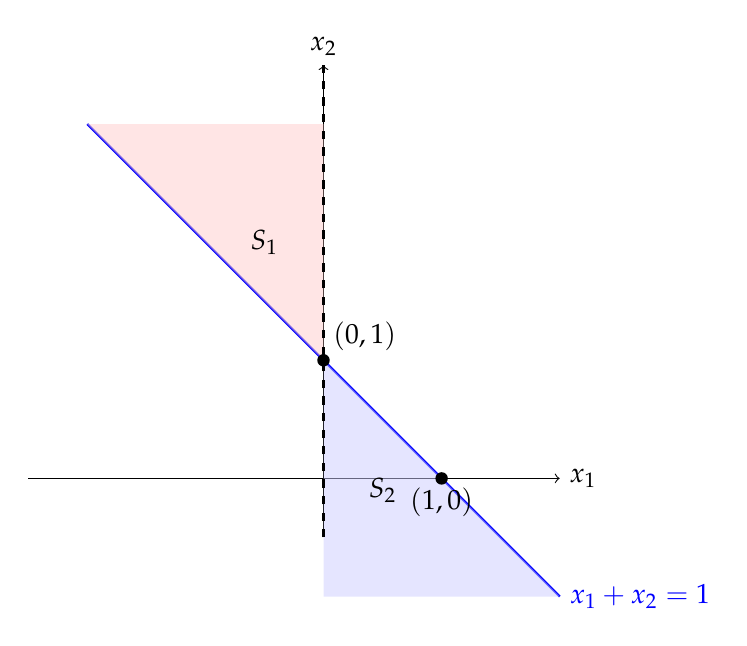
\begin{tikzpicture}[scale=1.5]
    % Draw axes
    \draw[->] (-2.5,0) -- (2,0) node[right] {$x_1$};
    \draw[->] (0,-0.5) -- (0,3.5) node[above] {$x_2$};
        
    % Draw the line x_1 + x_2 = 1
    \draw[thick, blue] (-2,3) -- (2,-1) node[right] {$x_1 + x_2 = 1$};
        
    % Shade S_1 (left region: x_1 <= 0 and x_1 + x_2 >= 1)
    % This is the unbounded region to the upper-left
    \fill[red!20, opacity=0.5] (0,1) -- (0,3) -- (-2,3) -- cycle;
        
    % Shade S_2 (right region: x_1 >= 0 and x_1 + x_2 <= 1)
    % This is a triangle with vertices (0,0), (1,0), (0,1)
    \fill[blue!20, opacity=0.5] (0,0) -- (0,1) -- (2,-1)-- (0,-1) -- cycle;
        
    % Draw boundary lines more clearly
    \draw[thick, dashed] (0,-0.5) -- (0,3.5);
        
    % Mark important points
    \fill (0,1) circle (1.5pt) node[above right] {$(0,1)$};
    \fill (1,0) circle (1.5pt) node[below] {$(1,0)$};
        
    % Label regions
    \node at (-0.5,2) {$S_1$};
    \node at (0.5,-0.1) {$S_2$};
\end{tikzpicture}
\end{center}

\item[(b)]

The constraints defining $S$ can be combined using a product form.

Note that the two regions correspond to

\[
(x_1 \le 0 \text{ and } x_1 \ge -x_2+1)
\]
or
\[
(x_1 \ge 0 \text{ and } x_1 \le -x_2+1).
\]

This can be written as

\[
x_1(x_1 + x_2 -1) \le 0.
\]

Expanding,

\[
q(\vec{x}) = x_1^2 + x_1x_2 - x_1.
\]

Now write this in quadratic form

\[
q(\vec{x}) = \vec{x}^T A \vec{x} + 2\vec{b}^T\vec{x} + c.
\]

Matching coefficients,

\[
A =
\begin{bmatrix}
1 & \tfrac12 \\
\tfrac12 & 0
\end{bmatrix},
\qquad
\vec{b} =
\begin{bmatrix}
-\tfrac12 \\
0
\end{bmatrix},
\qquad
c=0.
\]


\item[(c)]

The convex hull is simply the entire plane, i.e., $\text{conv}(S) = \mathbb{R}^2$.

\item[(d)]

The feasible set is

\[
S_1 =
\{\vec{x}\in\mathbb{R}^2 \mid x_1 \ge -x_2+1,\; x_1\le0\}.
\]

\begin{enumerate}

\item[(i)]

\[
f(\vec{x})=(x_1+1)^2+(x_2-3)^2
\]

The unconstrained minimizer occurs at

\[
(-1,3).
\]

Check feasibility:

\[
x_1=-1 \le0,
\]

\[
-1 \ge -3+1=-2
\]

which is satisfied.

Thus the point lies in $S_1$.

\medskip
Optimal point:

\[
\vec{x}^\star = (-1,3).
\]

Active constraints: none.

\bigskip

\item[(ii)]

\[
f(\vec{x})=(x_1+2)^2+(x_2-2)^2
\]

Unconstrained minimizer:

\[
(-2,2).
\]

Check feasibility:

\[
-2 \le0
\]

but

\[
-2 \ge -2+1=-1
\]

is false.

Thus the optimum lies on the boundary
\[
x_1 = -x_2+1.
\]

Substitute $x_1=1-x_2$:

\[
f(x_2) = (3-x_2)^2 + (x_2-2)^2.
\]

Differentiate:

\[
f'(x_2)=4x_2-10.
\]

Setting to zero gives

\[
x_2=2.5.
\]

Thus

\[
x_1 = 1-2.5 = -1.5.
\]

\medskip
Optimal point:

\[
\vec{x}^\star=(-1.5,\,2.5).
\]

Active constraint:

\[
x_1=-x_2+1.
\]

\bigskip

\item[(iii)]

\[
f(\vec{x}) = x_1^2 + x_2^2.
\]

Unconstrained minimizer:

\[
(0,0).
\]

Check feasibility:

\[
0 \le 0
\]

but

\[
0 \ge 1
\]

is false.

Thus the optimum lies on the boundary $x_1=-x_2+1$.

Substitute $x_1=1-x_2$:

\[
f(x_2)=(1-x_2)^2+x_2^2
\]

\[
=1-2x_2+2x_2^2.
\]

Differentiate:

\[
f'(x_2)=4x_2-2.
\]

Setting to zero gives

\[
x_2=\tfrac12.
\]

Thus

\[
x_1=\tfrac12.
\]

\medskip
Optimal point:

\[
\vec{x}^\star=(0.5,\,0.5).
\]

Active constraint:

\[
x_1=-x_2+1.
\]

\end{enumerate}

\end{enumerate}

%----------------------------------------------------------------------------------------

\newpage
\section*{Problem 4. Quadratics and Least Squares}

Consider $f: \mathbb{R}^2 \to \mathbb{R}$ defined by $f(\vec{w})=\vec{w}^{\top}A\vec{w}-2\vec{b}^{\top}\vec{w}+c$ with $A\in\mathbb{S}_{+}^{2}$.
\begin{enumerate}

\item[(a)] Assume $c = 0$, and assume that setting $\nabla f(\vec{w}) = 0$ allows us to find the unique minimizer. Give a concrete example of a matrix $A \succ 0$ and a vector $\vec{b}$ such that the point

\[
\vec{w}^\star =
\begin{bmatrix}
-1 \\
1
\end{bmatrix}
\]

is the unique minimizer of the quadratic function $f(\vec{w})$.

\item[(b)] Assume $c = 0$. Give a concrete example of a matrix $A \succeq 0$, and a vector $\vec{b}$ such that the quadratic function $f(\vec{w})$ has infinitely many minimizers and all of them lie on the line $w_1 + w_2 = 0$.

\item[(c)] Assume $c = 0$. Let

\[
\vec{w} =
\begin{bmatrix}
1 \\
0
\end{bmatrix}.
\]

Give a concrete example of a non-zero matrix $A \succeq 0$ and a vector $\vec{b}$ such that the quadratic function $f(\alpha \vec{w})$ tends to $-\infty$ as $\alpha \to \infty$.

\item[(d)] Say that we have the data set $\{(\vec{x}_i, y_i)\}_{i=1,...,n}$ of data points $\vec{x}_i \in \mathbb{R}^d$ and values $y_i \in \mathbb{R}$.

Define

\[
X =
\begin{bmatrix}
\vec{x}_1 \\
\vdots \\
\vec{x}_n
\end{bmatrix},
\quad
\vec{y} =
\begin{bmatrix}
y_1 \\
\vdots \\
y_n
\end{bmatrix}.
\]

In terms of $X$ and $\vec{y}$, find a matrix $A$, a vector $\vec{b} \in \mathbb{R}^d$ and a scalar $c$, so that we can express the sum of the square losses

\[
\sum_{i=1}^{n} ( \vec{w}^T \vec{x}_i - y_i )^2
\]

as the quadratic function

\[
f(\vec{w}) = \vec{w}^T A \vec{w} - 2\vec{b}^T \vec{w} + c.
\]

\item[(e)]

The discussion explains the behavior of quadratic minimization problems compared with least-squares problems.
For a general quadratic objective function:

\begin{enumerate}
\item[(i)] It can have a unique minimizer when the matrix $A \succ 0$ (the function is strictly convex).

\item[(ii)] It can have infinitely many minimizers when $A \succeq 0$ but is not full rank, so the objective is convex but not strictly convex.

\item[(iii)] It can be unbounded from below if $A$ has a direction in which the quadratic term vanishes while the linear term dominates.
\end{enumerate}

However, for the least-squares problem

\[
f(\vec w)=\|X\vec w-\vec y\|_2^2
\]

the objective is always nonnegative, so it cannot be unbounded from below.

Multiple minimizers occur only when

\[
\nabla f(\vec w^\star)=2X^TX\vec w^\star-2X^T\vec y=0
\]

has infinitely many solutions, which happens when $X^TX$ is not full rank. This occurs when

\[
\text{rank}(X^TX)=\text{rank}(X)<d,
\]

meaning the data points $\{\vec x_i\}$ do not span $\mathbb{R}^d$.

Thus the least-squares problem can have a unique solution or infinitely many solutions, but it cannot be unbounded below.


\end{enumerate}

\subsection*{Answer}

\begin{enumerate}

\item[(a)]

We need a matrix $A \succ 0$ and vector $\vec b$ such that the unique minimizer of
\[
f(\vec w)=\vec w^T A \vec w - 2\vec b^T \vec w
\]
is
\[
\vec w^\star=
\begin{bmatrix}
-1\\
1
\end{bmatrix}.
\]

The gradient is
\[
\nabla f(\vec w)=2A\vec w-2\vec b.
\]

Setting $\nabla f(\vec w)=0$ gives the optimality condition
\[
A\vec w^\star=\vec b.
\]

Choose a simple positive definite matrix
\[
A=I=
\begin{bmatrix}
1 & 0\\
0 & 1
\end{bmatrix}.
\]

Then
\[
\vec b=A\vec w^\star=
\begin{bmatrix}
-1\\
1
\end{bmatrix}.
\]

\item[(b)]

We want $A\succeq0$ and infinitely many minimizers lying on
\[
w_1+w_2=0.
\]

The optimality condition is again
\[
A\vec w=\vec b.
\]

Choose
\[
A=
\begin{bmatrix}
1&1\\
1&1
\end{bmatrix}.
\]

This matrix has eigenvalues $2$ and $0$, so $A\succeq0$ and $\operatorname{rank}(A)=1$.

Let
\[
\vec b=
\begin{bmatrix}
0\\
0
\end{bmatrix}.
\]

Then the optimality condition becomes
\[
A\vec w=0.
\]

Compute
\[
A\vec w=
\begin{bmatrix}
1&1\\
1&1
\end{bmatrix}
\begin{bmatrix}
w_1\\
w_2
\end{bmatrix}
=
\begin{bmatrix}
w_1+w_2\\
w_1+w_2
\end{bmatrix}.
\]

Thus
\[
w_1+w_2=0.
\]

Hence all minimizers lie on the line $w_1+w_2=0$, and there are infinitely many.

\medskip
One valid example is
\[
A=
\begin{bmatrix}
1&1\\
1&1
\end{bmatrix},
\quad
\vec b=
\begin{bmatrix}
0\\
0
\end{bmatrix}.
\]

\bigskip

\item[(c)]

Let
\[
\vec w=
\begin{bmatrix}
1\\
0
\end{bmatrix}.
\]

We want $A\succeq0$ (nonzero) and $\vec b$ such that
\[
f(\alpha \vec w)\to -\infty \quad \text{as } \alpha\to\infty.
\]

Choose
\[
A=
\begin{bmatrix}
0&0\\
0&1
\end{bmatrix}.
\]

This matrix is positive semidefinite and nonzero.

Let
\[
\vec b=
\begin{bmatrix}
1\\
0
\end{bmatrix}.
\]

Now compute

\[
f(\alpha \vec w)
=
(\alpha \vec w)^T A (\alpha \vec w)
-
2\vec b^T(\alpha \vec w).
\]

Since
\[
\alpha\vec w=
\begin{bmatrix}
\alpha\\
0
\end{bmatrix},
\]

we get

\[
(\alpha\vec w)^T A (\alpha\vec w)=0
\]

because $A_{11}=0$.

Also

\[
\vec b^T(\alpha\vec w)=\alpha.
\]

Thus

\[
f(\alpha\vec w)=-2\alpha.
\]

Therefore

\[
f(\alpha\vec w)\to -\infty
\quad \text{as } \alpha\to\infty.
\]

\bigskip

\item[(d)]

The least squares objective is

\[
\sum_{i=1}^n (\vec w^T \vec x_i - y_i)^2.
\]

Let

\[
X=
\begin{bmatrix}
\vec x_1^T\\
\vdots\\
\vec x_n^T
\end{bmatrix},
\qquad
\vec y=
\begin{bmatrix}
y_1\\
\vdots\\
y_n
\end{bmatrix}.
\]

Then

\[
\vec w^T\vec x_i
\]

is the $i$-th component of $X\vec w$, so

\[
\sum_{i=1}^n (\vec w^T\vec x_i-y_i)^2
=
\|X\vec w-\vec y\|_2^2.
\]

Expand:

\[
(X\vec w-\vec y)^T(X\vec w-\vec y).
\]

\[
=
\vec w^T X^T X \vec w
-
2\vec y^T X \vec w
+
\vec y^T \vec y.
\]

Since

\[
\vec y^T X \vec w=(X^T\vec y)^T\vec w,
\]

we can write

\[
f(\vec w)=\vec w^T A \vec w-2\vec b^T\vec w+c
\]

with

\[
A=X^TX,
\]

\[
\vec b=X^T\vec y,
\]

\[
c=\vec y^T\vec y.
\]

\bigskip

\item[(e)]

I have read and understood the discussion above.

\end{enumerate}
%----------------------------------------------------------------------------------------

\newpage
\section*{Problem 5. Direction of Steepest Ascent.}
\begin{enumerate}

\item[(a)] Let us define the rate of change of the function $f(\vec{x})$ at the point $\vec{x}$ along an arbitrary unit vector $\vec{u}$ as

\[
D_{\vec{u}} f(\vec{x}) =
\lim_{h \to 0}
\frac{f(\vec{x} + h\vec{u}) - f(\vec{x})}{h}.
\]

We call this the directional derivative. Show that the directional derivative can be equivalently expressed as

\[
D_{\vec{u}} f(\vec{x}) = \vec{u}^T [\nabla f(\vec{x})].
\]

HINT: Use Taylor approximation of the function around the point $\vec{x}$ and evaluate it at the point $\vec{x} + h\vec{u}$.

\item[(b)] Show that

\[
\frac{\nabla f(\vec{x})}{\|\nabla f(\vec{x})\|_2}
=
\arg\max_{\|\vec{u}\|_2 = 1}
\vec{u}^T [\nabla f(\vec{x})].
\]

\end{enumerate}

\subsection*{Answer}
\begin{enumerate}

\item[(a)]

The directional derivative of $f$ at $\vec{x}$ along a unit vector $\vec{u}$ is defined as

\[
D_{\vec{u}} f(\vec{x}) =
\lim_{h\to 0} \frac{f(\vec{x}+h\vec{u})-f(\vec{x})}{h}.
\]

Using the first-order Taylor expansion of $f$ around $\vec{x}$,

\[
f(\vec{x}+h\vec{u}) =
f(\vec{x}) + h \nabla f(\vec{x})^T \vec{u} + o(h),
\]

where $o(h)/h \to 0$ as $h \to 0$.

Substituting into the definition of the directional derivative,

\[
D_{\vec{u}} f(\vec{x})
=
\lim_{h\to0}
\frac{f(\vec{x}) + h\nabla f(\vec{x})^T\vec{u} + o(h) - f(\vec{x})}{h}.
\]

Simplifying,

\[
D_{\vec{u}} f(\vec{x})
=
\lim_{h\to0}
\left(
\nabla f(\vec{x})^T\vec{u} + \frac{o(h)}{h}
\right).
\]

Since $\frac{o(h)}{h}\to0$,

\[
D_{\vec{u}} f(\vec{x}) = \nabla f(\vec{x})^T \vec{u}.
\]


\item[(b)]

From part (a), the rate of change of $f$ in direction $\vec{u}$ is

\[
D_{\vec{u}} f(\vec{x}) = \vec{u}^T \nabla f(\vec{x}),
\]

where $\|\vec{u}\|_2 = 1$.

By the Cauchy–Schwarz inequality,

\[
\vec{u}^T \nabla f(\vec{x})
\le
\|\vec{u}\|_2 \, \|\nabla f(\vec{x})\|_2.
\]

Since $\|\vec{u}\|_2 = 1$,

\[
\vec{u}^T \nabla f(\vec{x})
\le
\|\nabla f(\vec{x})\|_2.
\]

Equality holds when $\vec{u}$ is parallel to $\nabla f(\vec{x})$, i.e.,

\[
\vec{u} =
\frac{\nabla f(\vec{x})}{\|\nabla f(\vec{x})\|_2}.
\]

Therefore the direction that maximizes the directional derivative is

\[
\arg\max_{\|\vec{u}\|_2=1} \vec{u}^T \nabla f(\vec{x})
=
\frac{\nabla f(\vec{x})}{\|\nabla f(\vec{x})\|_2}.
\]

Thus the gradient points in the direction of steepest ascent.

\end{enumerate}
%----------------------------------------------------------------------------------------
\newpage
\section*{Problem 6. Gradient Descent Algorithm.}


\begin{enumerate}

\item[(a)] Consider $f(x) = \frac{1}{2}(x - 2)^2$, and assume that we use the gradient descent algorithm

\[
x_{k+1} = x_k - \eta \nabla f(x_k) \quad \forall k \ge 0,
\]

with some random initialization $x_0$, where $\eta > 0$ is the step size (or the learning rate) of the algorithm.

Write $(x_k - 2)$ in terms of $(x_0 - 2)$, and show that $x_k$ converges to $2$, which is the unique minimizer of $f$, when $\eta = 0.2$.

\item[(b)] Let $\alpha, \beta \in \mathbb{R}$ and that for all $\eta$ such that $\alpha < \eta < \beta$, the gradient descent algorithm converges to $2$ from all possible initializations in $\mathbb{R}$.

What are the smallest $\alpha$ and the largest $\beta$?

After you determine $\alpha, \beta$, answer the following.

(i) $\eta = \alpha$

(ii) $\eta = \beta$

(iii) $\eta > \beta$

\item[(c)] Now assume that we use the gradient descent algorithm to minimize

\[
f(\vec{x}) =
\frac{1}{2}\|A\vec{x} - \vec{b}\|_2^2
\]

for some $A \in \mathbb{R}^{m\times n}$ and $\vec{b} \in \mathbb{R}^m$, where $A$ has full column rank.

First compute $\nabla f(\vec{x})$.

Note that $(A^T A)^{-1}A^T \vec{b}$ is the solution to the least-squares problem, and $(\vec{x}_k - (A^T A)^{-1}A^T\vec{b})$ is the distance from the solution at time $k$.

Write

\[
(\vec{x}_k - (A^T A)^{-1}A^T\vec{b})
\]

in terms of

\[
(\vec{x}_0 - (A^T A)^{-1}A^T\vec{b}).
\]

\item[(d)] Now consider

\[
f(\vec{x}) =
\frac{1}{2}\|A\vec{x} - \vec{b}\|_2^2
+
\frac{1}{2}\lambda \|\vec{x}\|_2^2
\]

for some $A \in \mathbb{R}^{m\times n}$, $\vec{b} \in \mathbb{R}^m$, and $\lambda \in \mathbb{R}$, where $A$ has full column rank and $\lambda \ge 0$.

Suppose we solve this problem via gradient descent with step-size

\[
\eta = \frac{1}{\sigma_1^2 + \lambda}
\]

where $\sigma_1$ is the maximum singular value of $A$.

Show the gradient descent converges.

\end{enumerate}

\subsection*{Answer}

\begin{enumerate}

\item[(a)]

We have
\[
f(x) = \frac{1}{2}(x-2)^2.
\]

The gradient is

\[
\nabla f(x) = x-2.
\]

The gradient descent update becomes

\[
x_{k+1} = x_k - \eta(x_k-2).
\]

Rewrite the recursion relative to the optimum:

\[
x_{k+1}-2 = x_k-2 - \eta(x_k-2).
\]

\[
x_{k+1}-2 = (1-\eta)(x_k-2).
\]

Applying this recursively gives

\[
x_k - 2 = (1-\eta)^k (x_0-2).
\]

If $\eta = 0.2$, then

\[
|1-\eta| = 0.8 < 1.
\]

Thus

\[
(1-\eta)^k \to 0 \quad \text{as } k \to \infty,
\]

so

\[
x_k \to 2.
\]

Hence gradient descent converges to the unique minimizer $x^\star = 2$.

\item[(b)]

From part (a),

\[
x_k - 2 = (1-\eta)^k (x_0-2).
\]

For convergence we need

\[
|1-\eta| < 1.
\]

This gives

\[
-1 < 1-\eta < 1.
\]

Solving,

\[
0 < \eta < 2.
\]

Thus

\[
\alpha = 0, \qquad \beta = 2.
\]

Now consider the boundary cases.

(i) $\eta = \alpha = 0$

\[
x_{k+1} = x_k,
\]

so the algorithm never moves and does not converge unless $x_0=2$.

(ii) $\eta = \beta = 2$

\[
x_{k+1}-2 = - (x_k-2).
\]

Thus

\[
x_k-2 = (-1)^k (x_0-2),
\]

which oscillates and does not converge (unless $x_0=2$).

(iii) $\eta > \beta$

\[
|1-\eta| > 1.
\]

Hence

\[
|(1-\eta)^k| \to \infty,
\]

so the iterates diverge.

\item[(c)]

The objective function is

\[
f(\vec{x}) = \frac{1}{2}\|A\vec{x}-\vec{b}\|_2^2.
\]

The gradient is

\[
\nabla f(\vec{x}) = A^T(A\vec{x}-\vec{b}).
\]

Gradient descent update:

\[
\vec{x}_{k+1}
=
\vec{x}_k - \eta A^T(A\vec{x}_k-\vec{b}).
\]

Let

\[
\vec{x}^\star = (A^TA)^{-1}A^T\vec{b}.
\]

Since

\[
A^T(A\vec{x}^\star-\vec{b}) = 0,
\]

subtract $\vec{x}^\star$:

\[
\vec{x}_{k+1}-\vec{x}^\star
=
\vec{x}_k-\vec{x}^\star
-
\eta A^TA(\vec{x}_k-\vec{x}^\star).
\]

Thus

\[
\vec{x}_{k+1}-\vec{x}^\star
=
(I-\eta A^TA)(\vec{x}_k-\vec{x}^\star).
\]

Recursively,

\[
\vec{x}_k-\vec{x}^\star
=
(I-\eta A^TA)^k(\vec{x}_0-\vec{x}^\star).
\]

\item[(d)]

Now

\[
f(\vec{x}) =
\frac{1}{2}\|A\vec{x}-\vec{b}\|_2^2
+
\frac{1}{2}\lambda\|\vec{x}\|_2^2.
\]

The gradient is

\[
\nabla f(\vec{x}) =
A^T(A\vec{x}-\vec{b}) + \lambda \vec{x}.
\]

Thus

\[
\nabla f(\vec{x})
=
(A^TA+\lambda I)\vec{x} - A^T\vec{b}.
\]

Gradient descent update:

\[
\vec{x}_{k+1}
=
\vec{x}_k
-
\eta\left((A^TA+\lambda I)\vec{x}_k - A^T\vec{b}\right).
\]

The minimizer satisfies

\[
(A^TA+\lambda I)\vec{x}^\star = A^T\vec{b}.
\]

Subtract $\vec{x}^\star$:

\[
\vec{x}_{k+1}-\vec{x}^\star
=
(I-\eta(A^TA+\lambda I))(\vec{x}_k-\vec{x}^\star).
\]

Thus

\[
\vec{x}_k-\vec{x}^\star
=
(I-\eta(A^TA+\lambda I))^k
(\vec{x}_0-\vec{x}^\star).
\]

The eigenvalues of $A^TA$ are $\sigma_i^2$, so the eigenvalues of $(A^TA+\lambda I)$ are

\[
\sigma_i^2 + \lambda.
\]

The largest is

\[
\sigma_1^2 + \lambda.
\]

With step size

\[
\eta = \frac{1}{\sigma_1^2+\lambda},
\]

all eigenvalues of

\[
I-\eta(A^TA+\lambda I)
\]

lie in $[0,1)$.

Therefore

\[
(I-\eta(A^TA+\lambda I))^k \to 0,
\]

which implies

\[
\vec{x}_k \to \vec{x}^\star.
\]

Hence gradient descent converges.

\end{enumerate}
%----------------------------------------------------------------------------------------

\section*{Problem 7}

With whom did you work on this homework? List the names and SIDs of your group members.

NOTE: If you didn’t work with anyone, you can put “none” as your answer.

\subsection*{Answer}
none

%----------------------------------------------------------------------------------------

\end{document}